\documentclass{article}
\usepackage{graphicx} % new way of doing eps files
\usepackage{listings} % nice code layout
\usepackage[usenames]{color} % color
\definecolor{listinggray}{gray}{0.9}
\definecolor{graphgray}{gray}{0.7}
\definecolor{ans}{rgb}{1,0,0}
\definecolor{blue}{rgb}{0,0,1}
% \Verilog{title}{label}{file}
\graphicspath{ {H:/ELC3338/Team8/CompOrg_Spring2018_S1_Team8/images/} }
\newcommand{\Verilog}[3]{
  \lstset{language=Verilog}
  \lstset{backgroundcolor=\color{listinggray},rulecolor=\color{blue}}
  \lstset{linewidth=\textwidth}
  \lstset{commentstyle=\textit, stringstyle=\upshape,showspaces=false}
  \lstset{frame=tb}
  \lstinputlisting[caption={#1},label={#2}]{#3}
}


\author{Matthew Carrano and Breana Leal}
\title{Lab 4: Beginning to Decode}

\begin{document}
\maketitle

\section{Simplified Report}
The instr\_parse module uses both R and D format to break down the instruction code. The module parsed the instruction bits successfully and it is verified using four instruction codes provided in class.
The regfile module reads  data from the regData file into an array of registers. The module outputs............... When write\_data is HIGH data will be written to the registers. This action is verified through the simulation.

\section{Code}
\Verilog{Verilog code for implementing the instr\_parse module.}{code:adder}{../code/decode/instr_parse.v}



\Verilog{Verilog code for implementing the regfile module.}{code:mux}{../code/decode/regfile.v}


\section{Testbench}

\Verilog{Verilog code for implementing the instr\_parse testbench.}{code:adder}{../code/decode/instr_parse_test.v}


\Verilog{Verilog code for implementing the regfile testbench.}{code:mux}{../code/decode/regfile_test.v}

\begin{figure}[h]	
	\caption{Timing diagram for instr\_parse module test.}
	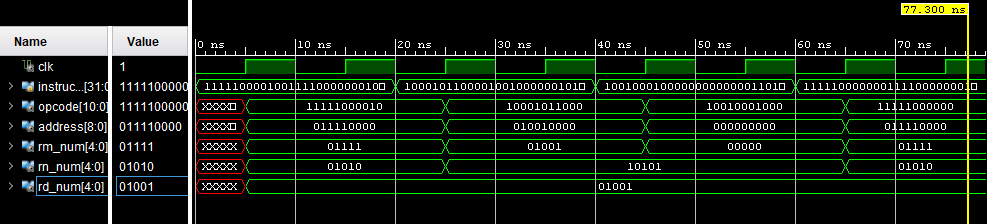
\includegraphics[width=\textwidth]{instr_parse_sim}
	
\end{figure}

\begin{figure}[h]	
	\caption{Timing diagram for regfile module test.}
	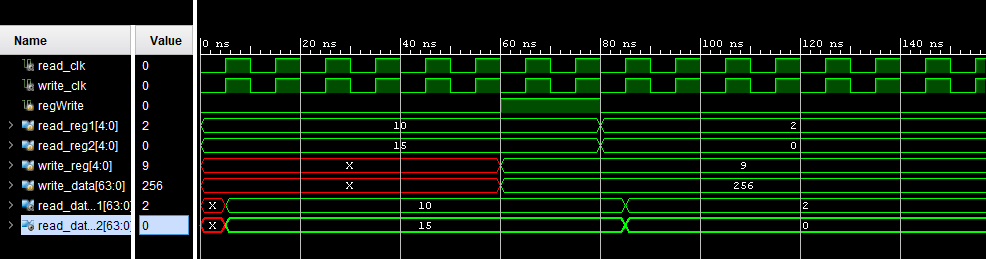
\includegraphics[width=\textwidth]{regfile_sim}
	\label{fig:fetchtest}
\end{figure}

The regfile simulation is working on the positive edge and 

\begin{figure}[h]	
	\caption{Modified Register File Data.}
	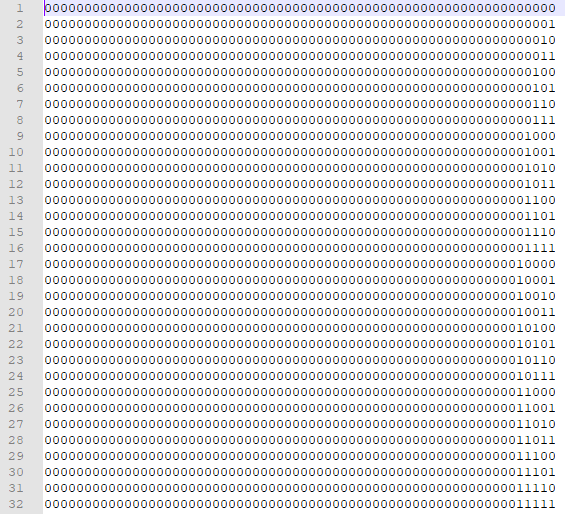
\includegraphics[width=\textwidth]{Modified_data}
	\label{fig:fetchtest}
\end{figure}

\section{Simulation}

\begin{figure}[h]	
	\caption{Timing diagram for instr\_parse module test.}
	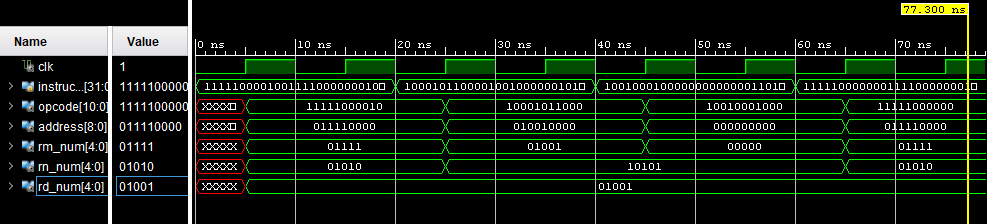
\includegraphics[width=\textwidth]{instr_parse_sim}

\end{figure}

\begin{figure}[h]	
	\caption{Timing diagram for regfile module test.}
	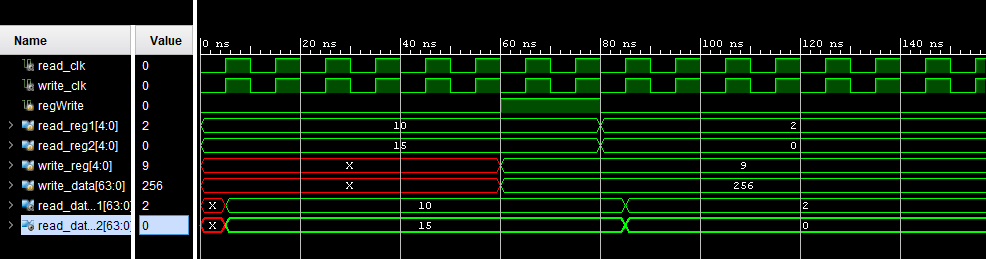
\includegraphics[width=\textwidth]{regfile_sim}
	\label{fig:fetchtest}
\end{figure}

The regfile simulation is working on the positive edge and 

\begin{figure}[h]	
	\caption{Modified Register File Data.}
	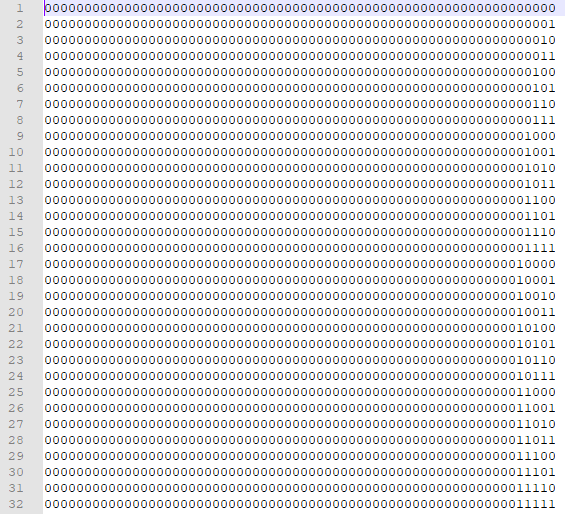
\includegraphics[width=\textwidth]{Modified_data}
	\label{fig:fetchtest}
\end{figure}


\end{document} 